
{The circuit is composed of three 2N3904 Bipolar Junction Transistors (BJTs), labeled as \( Q_1 \), \( Q_2 \), and \( Q_3 \), along with fourteen resistors and six electrolytic capacitors. The power supply \( V_{CC} \) provides a 10 V source, which is modulated by the sinusoidal signal source \( V_s \).}

{}

{}

\begin{figure}[H]
    \centering
    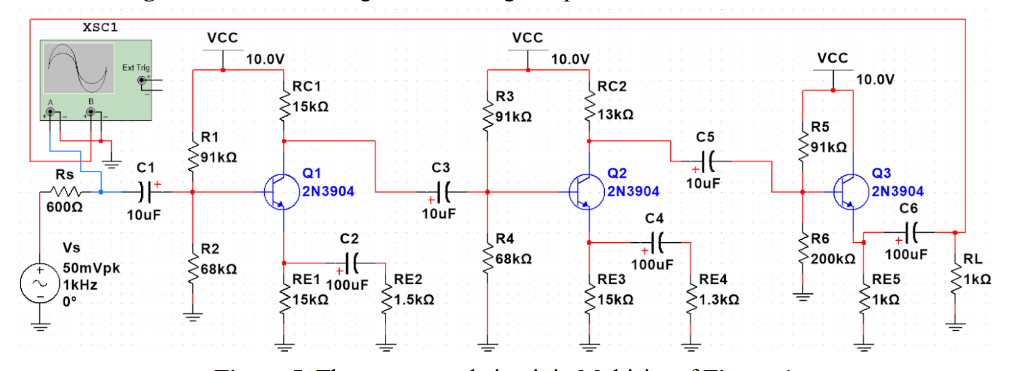
\includegraphics[width=16cm]{Pictures/Circuit.png}
    \caption{{Complete Circuit Diagram}}
    \label{circuit-dia}
\end{figure}
